%\graphicspath{{/Users/emiliendurif/Documents/prepa/sujets/DS/canne_robotise/}}

\vspace{-1cm}
\subsection{Présentation générale}
\vspace{-.5cm}
\subsubsection{Contexte}\label{contexte}


L'autofocus (AF) est le terme anglais pour désigner la mise au point
automatique. C'est une fonction qui permet la mise au point automatique
de certains systèmes optiques comme les appareils photo, leur permettant
de régler la netteté du sujet. Cette mise au point est réalisée grâce à
l'association d'un boitier et d'un objectif photographiques.

\begin{figure}[!htb]
\begin{center}
\begin{tabular}{ccc}
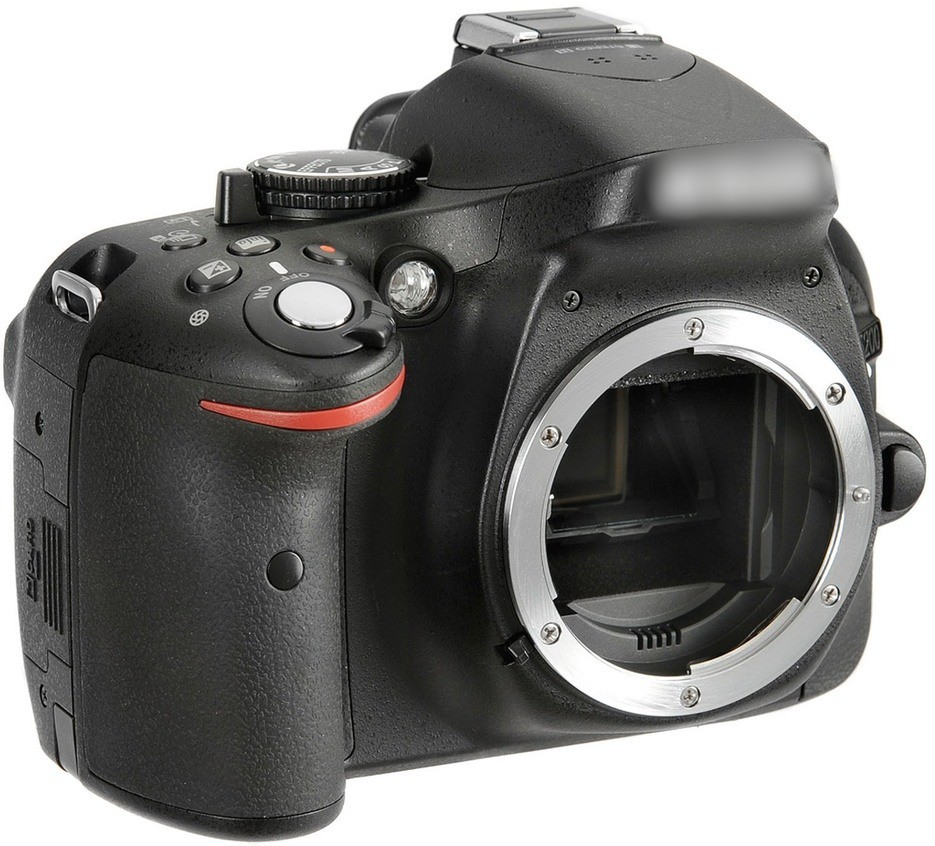
\includegraphics[width=0.25\textwidth]{images/image6.jpeg}
&

\includegraphics[width=0.21\textwidth]{images/image7.png}
&
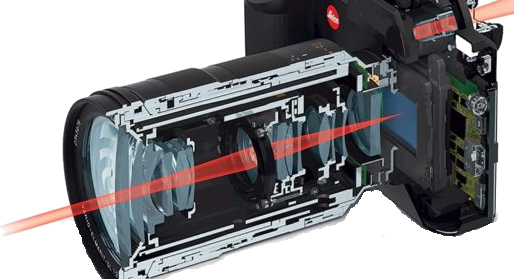
\includegraphics[width=0.35\textwidth]{images/image8.png}
\\
\textbf{boitier}& \textbf{objectif}& \textbf{boitier + objectif}
\end{tabular}
\caption{Boitier et objectif photographiques \label{fig1}}
\end{center}
\end{figure}
\vspace{-.5cm}


Le principe consiste à déplacer une lentille afin que les rayons de
l'image à photographier convergent sur le capteur. Si ce n'est pas le
cas, l'image sera floue. Sur la figure \ref{fig2}, la lentille est bien positionnée uniquement sur le schéma du milieu :
les rayons convergent parfaitement sur le capteur.


\begin{figure}[!htb]
\begin{center}
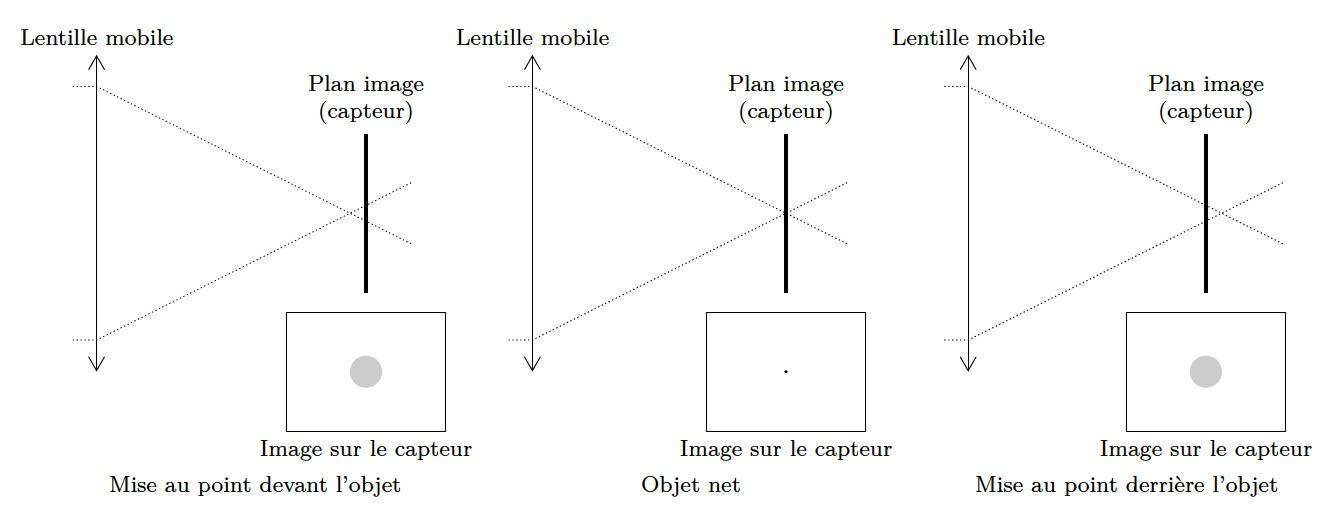
\includegraphics[width=0.8\textwidth]{images/image_fig2.jpg}
\caption{Principe de la mise au point (source :\url{http://www.pierretoscani.com/autofocus.html)} \label{fig2}}
\end{center}
\end{figure}

\FloatBarrier

\subsubsection{Mise en situation}\label{mise-en-situation}


Le mouvement de la lentille est donné par l'architecture représentée
figure \ref{fig3}

L'architecture détaillée est donnée en figure \ref{fig4}. La modélisation acausale
correspondante de l'objectif photographique est donnée figure \ref{fig5}.

\begin{figure}[!htb]
\begin{center}
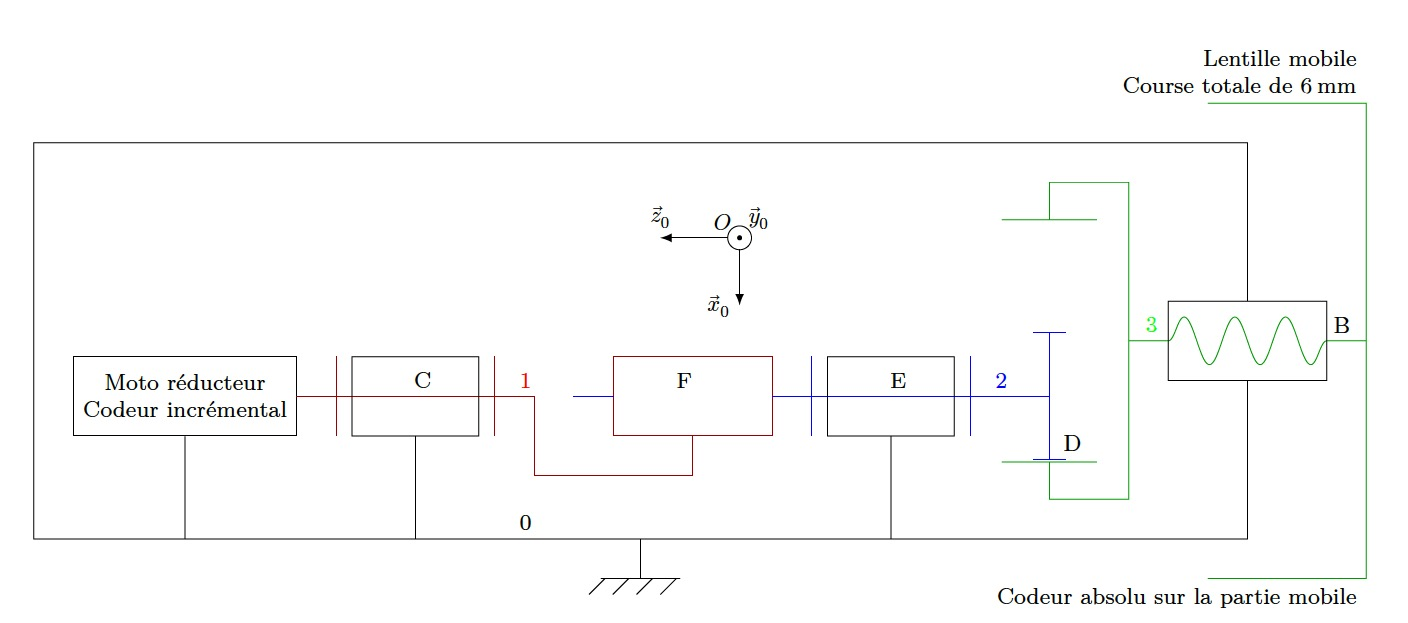
\includegraphics[width=1.0\textwidth]{images/image_fig3.jpg}
\caption{Architecture du dispositif de déplacement de la lentille \label{fig3}}
\end{center}
\end{figure}

\begin{figure}[!htb]
\begin{center}
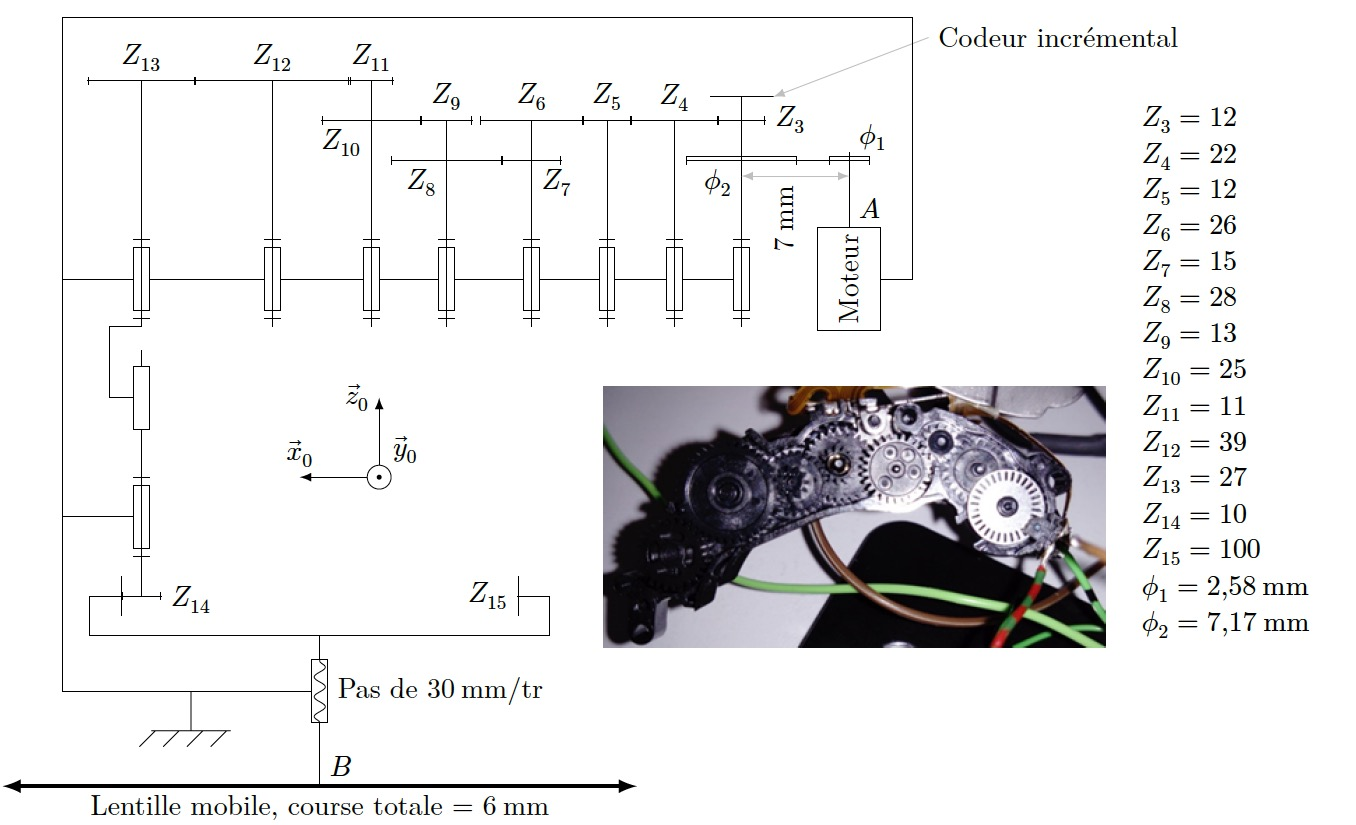
\includegraphics[width=1.0\textwidth]{images/image_fig4.jpg}
\caption{Schéma cinématique du mécanisme de déplacement de la lentille \label{fig4}}
\end{center}
\end{figure}

\begin{figure}[!htb]
\begin{center}
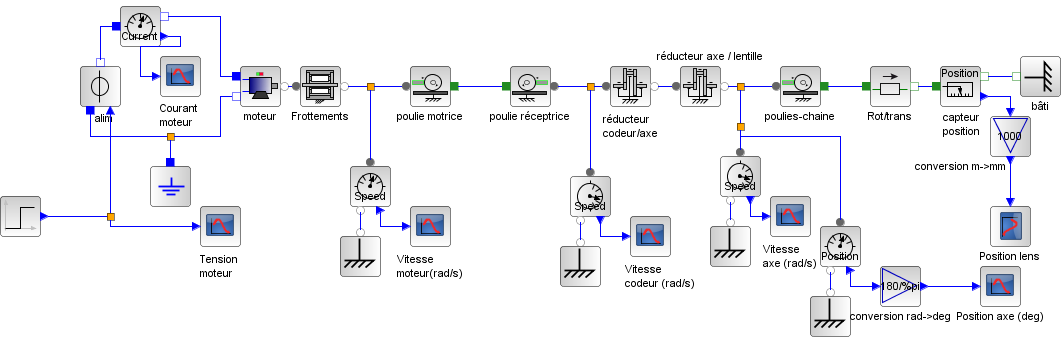
\includegraphics[width=1.0\textwidth]{images/image13.png}
\caption{Architecture du dispositif de déplacement de la lentille \label{fig5}}
\end{center}
\end{figure}

\FloatBarrier
\subsubsection{Extrait du cahier des charges}\label{extrait-du-cahier-des-charges}

\begin{figure}[!htb]
\begin{center}
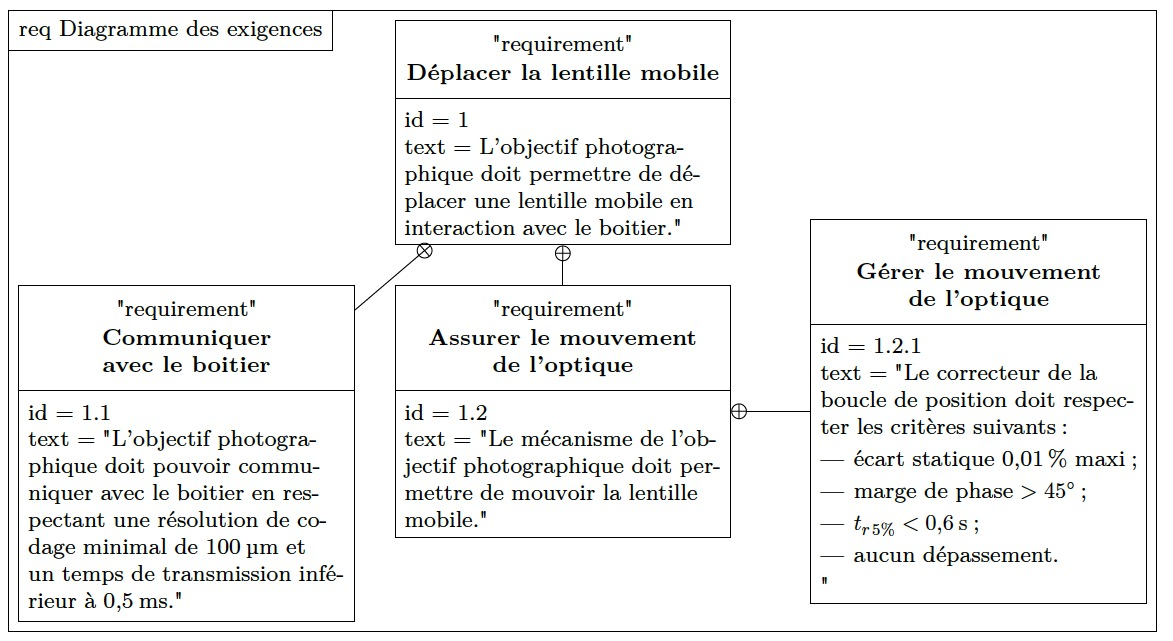
\includegraphics[width=0.8\textwidth]{images/image_fig6.jpg}
\caption{Exigences extraites du cahier des charges \label{fig6}}
\end{center}
\end{figure}

\subsubsection{Objectif ftnal}\label{objectif-ftnal}

Le sujet a pour but de modéliser, analyser et améliorer les performances
de l'objectif photographique. Pour cela, il comporte trois parties avec
comme buts :


\begin{itemize}
\item analyser l'architecture du système étudié et discuter de l'utilisation de capteurs pour remplir le cahier des charges.
\item Valider la structure permettant d'assurer le mouvement de l'optique.
\item Modéliser l'asservissement du système et vérifier les performances.
\end{itemize}

%
%\begin{itemize}
%\item
%  valider la communication entre le boitier et l'objectif photographique
%  permettant la mise au point et déter- miner la consigne qui doit être
%  envoyée par le boitier --- il est question de valider le temps de
%  communication qui doit être négligeable devant la dynamique du système
%  ;
%\item
%  modéliser la structure permettant d'« assurer le mouvement de
%  l'optique » --- cette partie permet de modéliser et de déterminer
%  numériquement les frottements au travers de mesures, ces grandeurs
%  sont fondamentales car les non linéarités vont fortement influencer la
%  commande ;
%\item
%  choisir et régler le correcteur permettant de « gérer le mouvement de
%  l'optique » --- cette partie permet de trouver le bon compromis de
%  réglage de la commande afin de respecter les critères du cahier des
%  charges.
%\end{itemize}


\subsection{Analyse structurelle du système}

\begin{objectif}
Analyser la structure de l'objectif photographique et en particulier la chaine fonctionnelle assurant l'autofocus.
\end{objectif}

La mise au point résulte de l'interaction entre le boitier (possédant un micro-controleur spécifique) où se situe
tout le traitement de numérisation de l'image (capteur CCD et programme
de mise au point) et l'objectif photographique qui permet de mouvoir la
lentille. Afin de réaliser correctement cette mise au point, il est
nécessaire que l'objectif photographique puisse communiquer avec tous
les boitiers compatibles en répondant aux exigences suivantes.

\begin{tabular}{|p{0.15\textwidth}|p{0.5\textwidth}|p{0.1\textwidth}|}
\hline 
\textbf{Exigence} & \textbf{Critère d'appréciation} & \textbf{Niveau} \\ 
\hline 
Id = « 1.1 » Communiquer avec le boitier & Temps de transmission d'un échange entre l'objectif photographique et le boitier & $0,5s$ \\ 
\cline{2-3}
& Résolution & $100\mu m$ \\ 
\hline 
\end{tabular} 


\begin{minipage}{0.4\textwidth}
Lorsque l'utilisateur appuie sur le déclencheur, l'objectif
photographique entre dans une phase d'initialisation durant laquelle la
lentille mobile figure \ref{fig4} se déplace de
la mise au point minimale à la mise au point infinie, ce qui correspond
à sa course totale.

L'utilisateur a la possibilité de contrôler sa mise au point dans la lunette à l'aide de collimateurs (figure ci-contre).
\end{minipage}
\begin{minipage}{0.6\textwidth}
\begin{center}
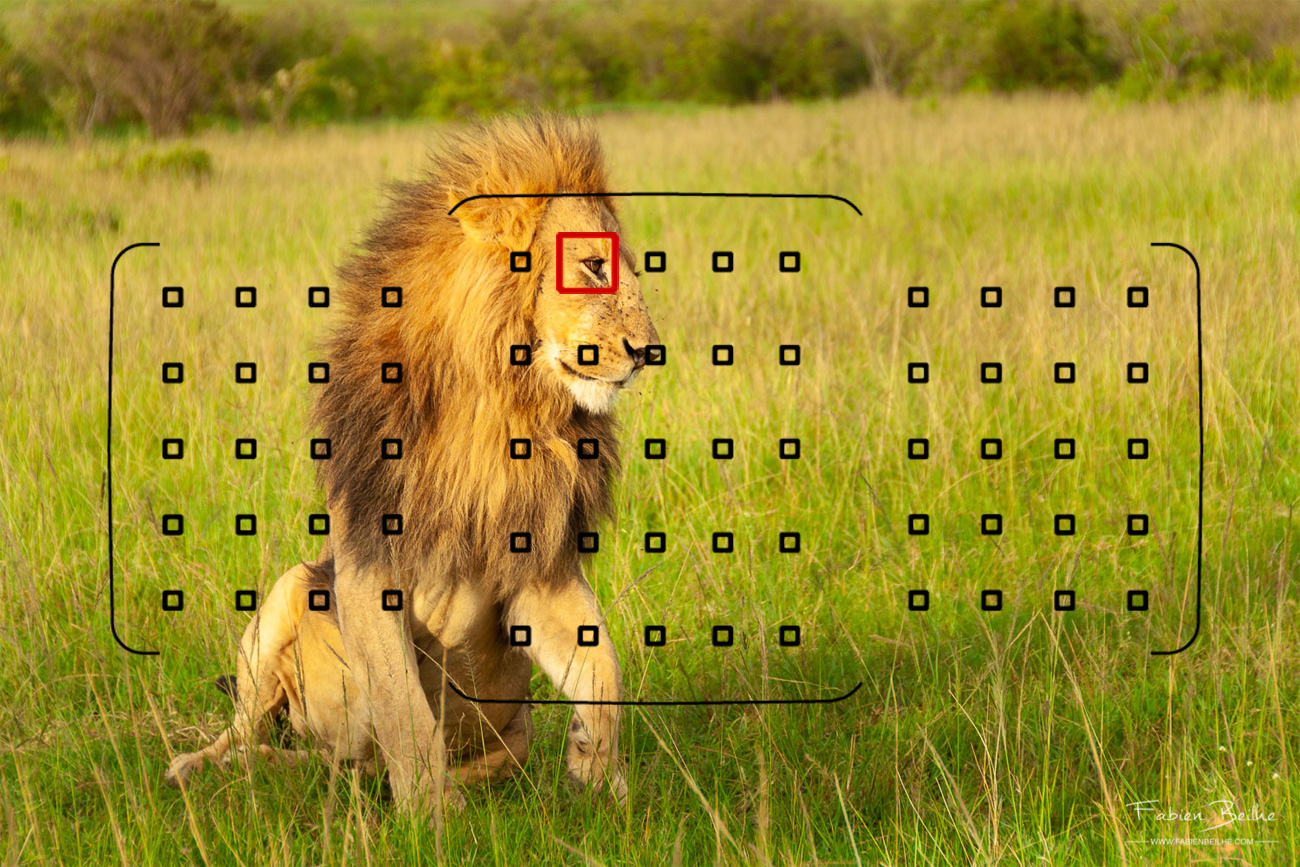
\includegraphics[width=0.7\textwidth]{images/collimateurs.jpg}
\end{center}
\end{minipage}

\begin{minipage}{0.4\textwidth}
L'objectif photographique est équipé de deux capteurs permettant de
mesurer le déplacement de la lentille :
\begin{itemize}
\item un codeur absolu linéaire 4bits, situé au niveau de la la lentille mobile permettant de connaître la position de la lentille mobile selon la direction $\overrightarrow{z}_0$ (figure \ref{fig4})
\item un codeur incrémental (monovoie, 30 impulsions par tour) relié au moteur par un dispositif poulies-courroie (figure \ref{fig4})
\end{itemize}
\end{minipage}
\begin{minipage}{0.6\textwidth}
\begin{center}
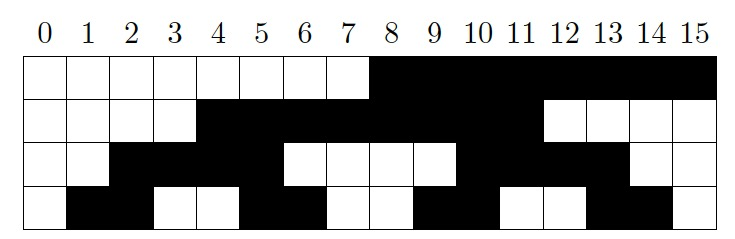
\includegraphics[width=0.9\textwidth]{images/absolu.jpg}\\
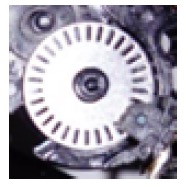
\includegraphics[width=0.2\textwidth]{images/relatif.jpg}
\end{center}
\end{minipage}

Dans les objectifs haut de gamme comme étudié ici, le moteur est inclus dans l'objectif. On peut trouver des moteurs pas-à-pas ou ultrasonique silencieux (gamme AP-S Nikon). Ici on considéra que c'est cette dernière technologie qui est utilisée. Elle est pilotée par un variateur ultrasonique spécifique délivrant une tension alternative de haute fréquence (40kHz) appliqué à un céramique piezo-électrique.


\question{A partir des données présentées dans la partie précédente compléter la chaine fonctionnelle relative à l'autofocus d'un appareil photo réflex.}

\question{Sur la modélisation multiphysique, repérer les parties acausales et les parties causales. Pour cela on surlignera en rouge ce qui représente la modélisation causale et en bleu ce qui représente la modélisation acausale.}


\question{Décrire en quelques phrases ce modèle et ce qu'il permet de représenter. En particulier en explicitera les grandeur physiques et la façon dont elles sont mesurées. On précisera également qu'elles sont les grandeurs imposées et mesurées.}

\question{Préciser les différences du point de vue de l'utilisation entre les codeurs absolus et relatifs.}


Pour obtenir une zone de mise au point la plus nette possible, il est
nécessaire que la résolution au niveau du positionnement de la lentille
mobile soit inférieure à $100\mu m$.

\question{Donner la résolution possible pour la course totale de la
lentille mobile avec le codeur absolu. Justifier que le codeur absolu ne
soit utilisé que lors de la phase d'initialisation de l'objectif
photographique.}


\question{Déterminer la relation entre le déplacement de la lentille mobile $d_l$ et la position angulaire du codeur incrémental $\theta_{rc}$. En déduire la résolution possible pour la course totale de
la lentille, si elle est déterminée en comptant les impulsions du codeur
incrémental sur les fronts montants.}

Dans la suite, la résolution sera prise égale à $5 \mu m$.

\question{En déduire le nombre de bits nécessaires pour coder
l'information « déplacement de la lentille mobile », si cette dernière
est donnée par le comptage du nombre d'impulsions au niveau du codeur
incrémental.}


\subsection{Validation de la structure permettant d'assurer le mouvement de l'optique}\label{validation-de-la-structure-permettant-dassurer-le-mouvement-de-loptique}

\begin{objectif}
Valider la structure qui permet de faire translater la lentille mobile
et de déterminer les différents paramètres du modèle multi-physique de
l'objectif photographique. On assimilera le moteur ultrasonique silencieux à une machine à courant continu (MCC).
Afin de vérifier et d'améliorer les performances de l'objectif
photographique, il est nécessaire de déterminer les différents
paramètres du modèle multi-physique donné précédemment. La démarche
adoptée ici est la suivante :

\begin{itemize}
\item
  détermination de l'équation de mouvement au niveau de la MCC (non demandée ici);
\item
  détermination des paramètres du modèle de la MCC ;
\item
  modélisation du frottement sec et du frottement visqueux.
  \end{itemize}
\end{objectif}

\subsubsection{Détermination du modèle de la machine à courant continu}

Afin d'identifier le modèle de la machine à courant continu, différents
essais à rotor bloqué et en charge à différentes vitesses sont
effectués. Ainsi, il est possible de déterminer expérimentalement les
paramètres du modèle multiphysique suivants :

\begin{minipage}{0.5\textwidth}
\textbf{Constantes du modèle :}
\begin{itemize}
\item la résistance d'induit, notée $R_m$ ;
\item l'inductance d'induit, notée $L_m$ ;
\item la constante de fcém, notée $K_e$ ;
\item la constante de couple, notée $K_T$ ;
\item le moment d'inertie ramené sur l'axe de la MCC, noté $J$ ;
\item le couple de frottement visqueux, noté $f$ ;
\end{itemize}

\end{minipage}
\begin{minipage}{0.5\textwidth}
\textbf{Variables du modèle : }
\begin{itemize}
\item courant de l'induit, noté $i_m(t)$ ;
\item tension de l'induit, noté $u_m(t)$ ;
\item tension de force contre-électromotrice, noté $e(t)$ ;
\item le couple total de frottement sec ramené sur l'axe de la MCC, noté $C_0(t)$ ;
\item la vitesse de rotation de l'axe de la MCC, noté $\omega_m(t)$ ;
\item le couple moteur de l'axe de la MCC, noté $C_m(t)$ ;
\end{itemize}
\textbf{Hypothèses : } On se placera dans les conditions de Heavyside avec les conditions initiales nulles.

\end{minipage}

\textbf{Modèle de connaissance :}
\begin{align*}
C_m(t)-C_0(t)-f\cdot \omega_m(t)=J\cdot\frac{d\omega_m(t)}{dt}\;\text{Equation de mouvement}\\
\\
u_m(t)=e(t)+L_m\frac{di_m(t)}{dt}+R_m\cdot i_m(t)\;\text{Equation électrique}\\
\\
e(t)=K_e\cdot \omega_m(t)\;\text{Equation électromécanique}\\\\
\\
C_m(t)=K_T\cdot i_m(t)\;\text{Equation électromécanique}\\.
\end{align*}

\question{Passer les équations du modèle de connaissance dans le domaine de Laplace.}

\question{On donne la structure du schéma bloc modélisant le moteur à courant continu. Compléter le schéma en précisant les fonctions de transfert et les variables.}

\begin{center}
\begin{large}
\begin{tikzpicture}
\sbEntree{E0}
\sbComp[4]{c2}{E0}
\sbRelier[$U_m(p)$]{E0}{c2}
\sbBloc[1]{b2}{}{c2}
\sbRelier{c2}{b2}
\sbBloc[4]{b3}{}{b2}
\sbRelier[]{b2}{b3}
%\sbComp[4]{c3}{b3}
\sbComph[6]{c3}{b3}
\sbDecaleNoeudy[-4]{c3}{E2}
\sbRelier[]{E2}{c3}
\sbBloc[7]{b4}{}{b3}
\sbRelier[]{b3}{c3}
\sbRelier{c3}{b4}
\sbSortie[5]{S}{b4}
\sbRelier[\hspace{.75cm}$\Omega_m(p)$]{b4}{S}
\sbDecaleNoeudy[4]{S}{v}
\sbBlocr[6]{b5}{}{v}
\sbRelieryx{b4-S}{b5}
\sbRelierxy[]{b5}{c2}
\end{tikzpicture}
\end{large}
\end{center}





Lors de l'essai de la machine à courant continu à rotor bloqué et sous tension d'induit réduite ($u_m(t)$) de $1,6 V$, le courant d'induit ($i_m(t)$) est mesuré. Les résultats sont donnés sur la figure \ref{fig9}.

\question{Exprimer sous ces conditions $I_m(p)$ en fonction de $U_m(p)$.}


\question{Donner l'expression de $U_m(p)$ et en déduire $I_m(p)$.}

\question{A l'aide de la figure \ref{fig9} et des résultats précédents, justifier la forme de la courbe à partir du modèle proposé.}

\question{Déterminer la résistance d'induit $R_m$ et de l'inductance d'induit $L_m$ à partir de l'essai à rotor bloqué et des équations précédentes.}

\begin{figure}[!htb]
\begin{center}
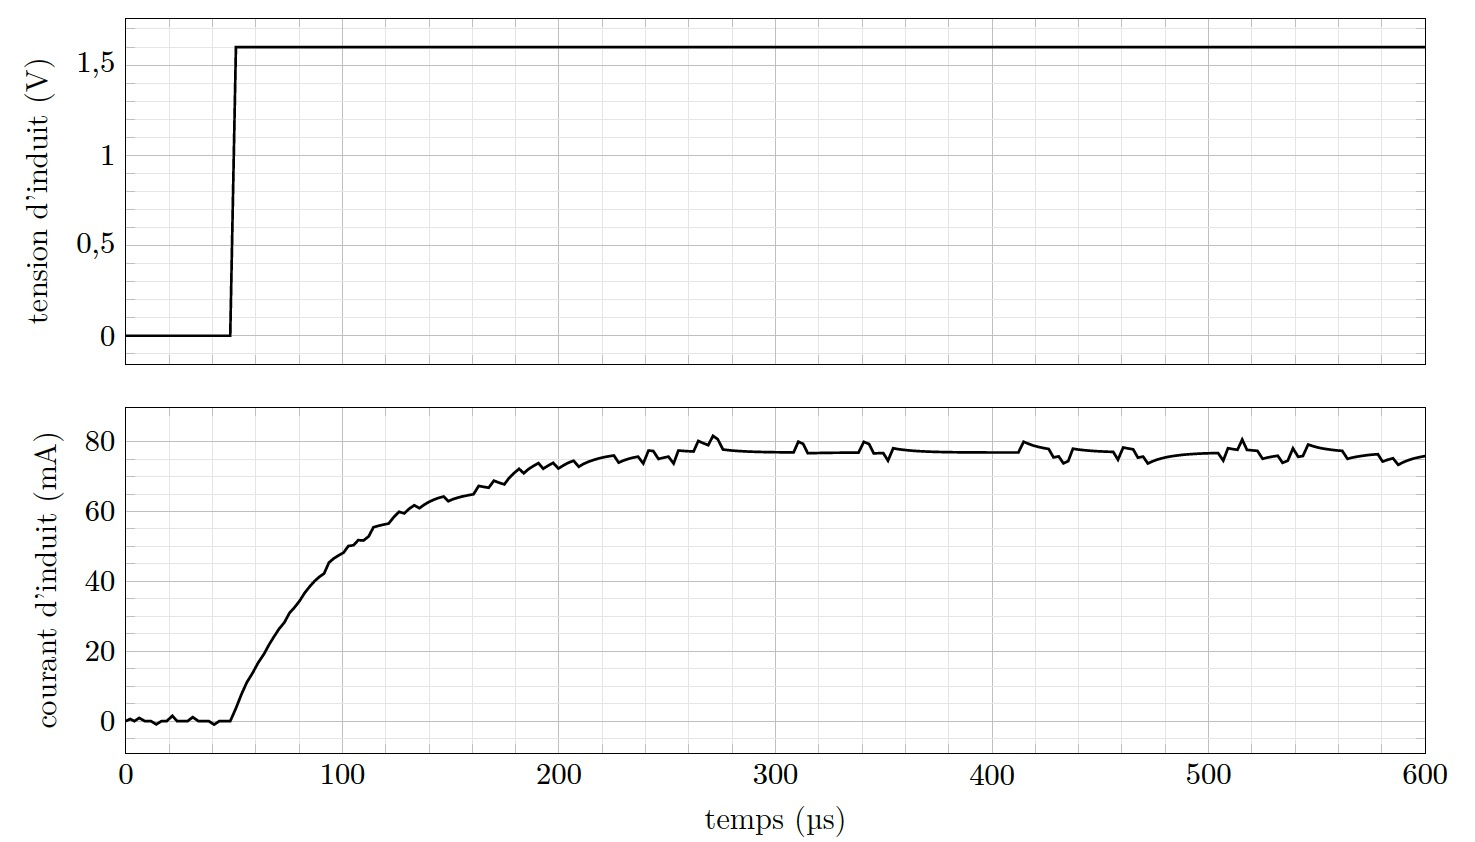
\includegraphics[width=0.9\textwidth]{images/image_fig9.jpg}
\caption{Résultats de l’essai de la MCC à rotor bloqué \label{fig9}}
\end{center}
\end{figure}


Plusieurs essais à vide avec des tension d'induit ($u_m(t)$) différentes ont permis de tracer la courbe de la
figure \ref{fig12}.

\question{Déterminer à partir de ces résultats la valeur numérique de la constante de fcém ($K_e$) que l'on supposera égale à la constante de couple ($K_T$).}

\begin{figure}[!htb]
\begin{center}
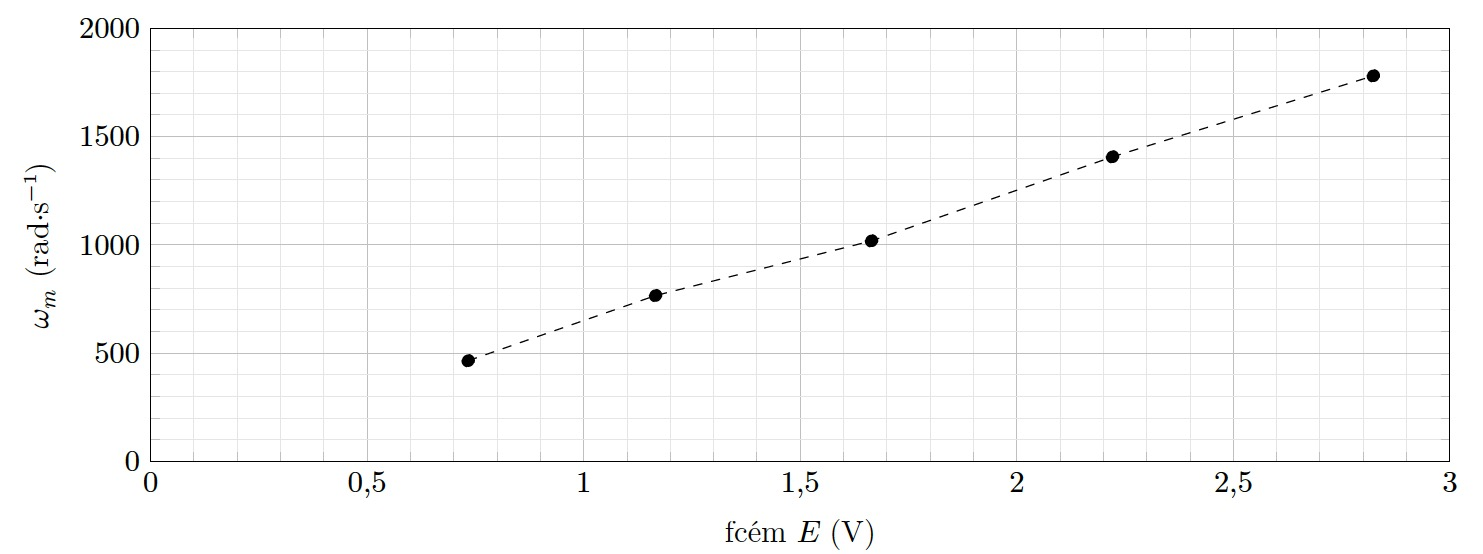
\includegraphics[width=0.9\textwidth]{images/image_fig12.jpg}
\caption{Mesures de vitesses angulaire du moteur en régime permanent pour différentes tensions d’induit \label{fig12}}
\end{center}
\end{figure}

\FloatBarrier
\subsubsection{Modélisation du frottement}

Le réglage de la lentille nécessite un asservissement en position. Dans ce cas le frottement qui induit une non-linéarité avec un seuil va perturber le système. Ainsi, il est primordial de quantifier les coefficient pour pouvoir
régler la commande. Des essais ont été réalisés sur un prototype pour déterminer les valeurs des couples de
frottement sec $C_0$ et visqueux $f$.

Quelle que soit la valeur trouvée précédemment, on prendra pour valeur de la constante de couple $K_T= 0,0019 N\cdot m\cdot A^{-1}$.

Différents essais sont effectués pour plusieurs tensions d'alimentation de la MCC d'amplitude ($u_0$). Les résultats sont donnés sur
la figure \ref{fig13}.

\begin{figure}[!htb]
\begin{center}
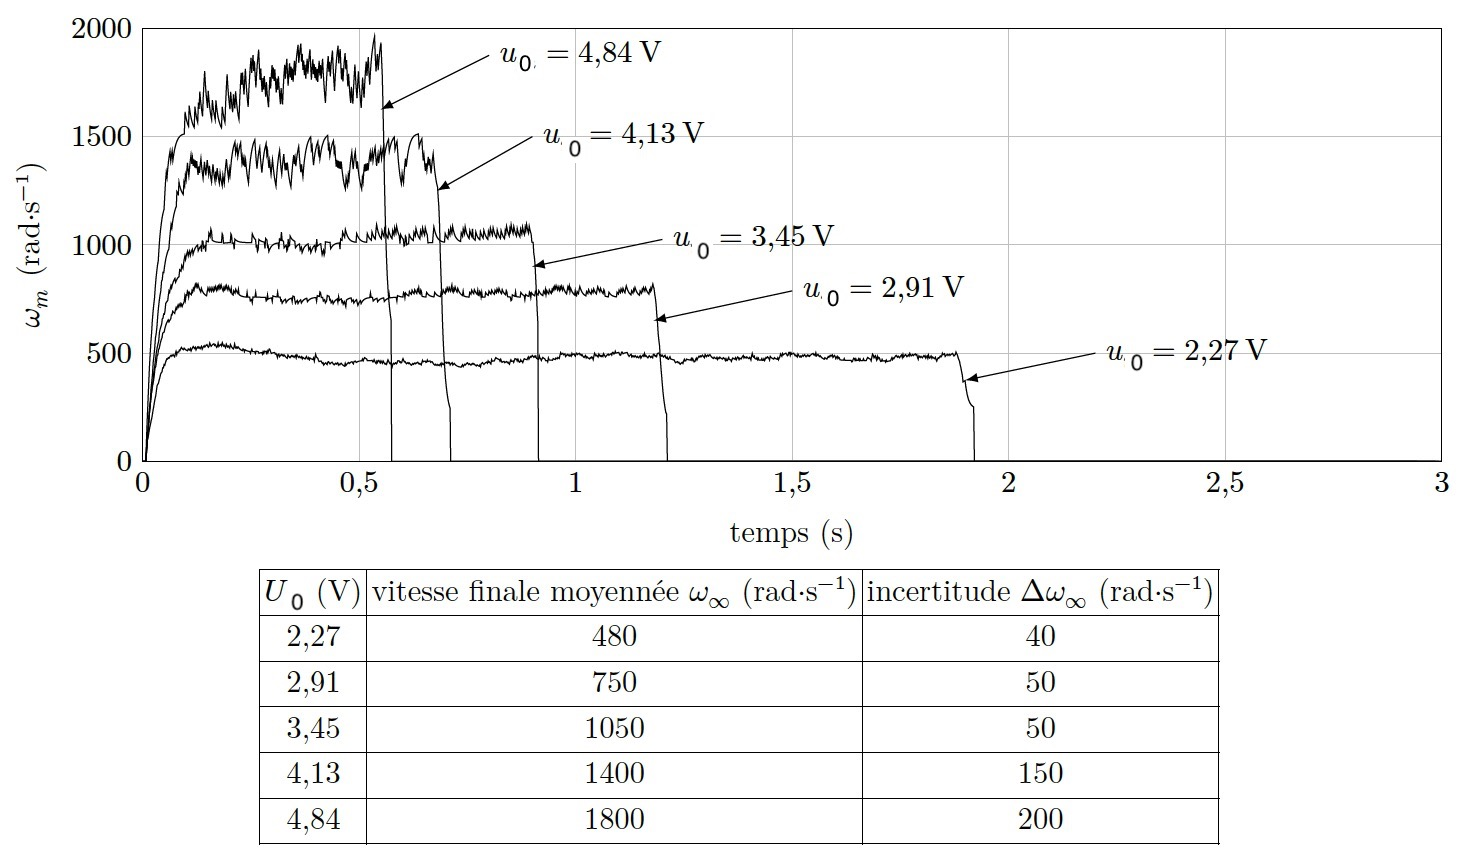
\includegraphics[width=0.9\textwidth]{images/image_fig13.jpg}
\caption{Mesures de vitesses angulaire du moteur pour différentes tensions d’induit \label{fig13}}
\end{center}
\end{figure}

\question{Déterminer l'expression de la vitesse de rotation de la MCC en régime permanent notée $\omega_{\infty}$ en fonction des paramètre $U_m$, $C_0$, $K_T$, $K_e$, $R_m$ et $f$.}



Le tableau de la figure \ref{fig13} donne la vitesse en régime permanent $\omega_{\infty}$ ainsi que l'incertitude sur la mesure $\Delta \omega_{\infty}$.

\question{Tracer sur le document réponse la courbe $\omega_{\infty}(U_m)$.}

\question{En déduire les valeurs numériques de $C_0$ et $f$.}

\question{Placer sur la courbe les incertitudes dues à la dispersion des mesures.}

\question{En tenant compte des incertitudes dans la mesure de vitesse, donner un encadrement de $C_0$ et de $f$.}


\subsection{Modélisation de l'asservissement permettant de "gérer le mouvement de l'optique"}

\begin{objectif}
Choisir et régler un correcteur afin de répondre aux exigences du cahier des charges
\end{objectif}

\begin{tabular}{|p{0.15\textwidth}|p{0.5\textwidth}|p{0.1\textwidth}|}
\hline 
\textbf{Exigence} & \textbf{Critère d'appréciation} & \textbf{Niveau} \\ 
\hline 
Id = « 1.2.2 » Gérer le mouvement de l'optique & Précision, erreur statique & $<0,1\%$ \\ 
\cline{2-3}
& Rapidité $t_{r5\%}$ & $0,6s$ maxi \\ 
\cline{2-3}
& Dépassement $D_1$ & aucun dépassement \\ 
\hline 
\end{tabular} 


Le réglage nécessite un compromis
entre les différents critères. Le frottement sec induit une difficulté
particulière car il impacte fortement la rapidité : si le gain en boucle
ouverte est trop faible le système ne pourra pas se mettre en mouvement,
si celui-ci est trop élevé, le système risque de devenir instable. La
suite du questionnement a pour but d'étudier comment trouver un bon
compromis.

Le modèle causal de l'objectif photographique dont les paramètres ont
été déterminés expérimentalement précédemment est donné figure \ref{fig14}. Il s'agit de l'asservissement du déplacement de la lentille (noté $D_l(p)$ dans le domaine de Laplace).

\begin{figure}[!htb]
\begin{center}
\begin{large}
\begin{tikzpicture}
\sbEntree{E0}
\sbBloc[3]{b0}{$K_a$}{E0}
\sbRelier[$D_c(p)$]{E0}{b0}
\sbComp[3]{c1}{b0}
\sbRelier{b0}{c1}
\sbBloc[4.5]{b1}{$C(p)$}{b0}
\sbRelier[$\varepsilon(p)$]{c1}{b1}
\sbComp[5.5]{c2}{b1}
\sbRelier[$U_m(p)$]{b1}{c2}
\sbBloc[1]{b2}{$A$}{c2}
\sbRelier{c2}{b2}
\sbBloc[1]{b3}{$B$}{b2}
\sbRelier{b2}{b3}
%\sbComp[4]{c3}{b3}
\sbComph{c3}{b3}
\sbDecaleNoeudy[-4]{c3}{E2}
\sbRelier[$C_0(p)$]{E2}{c3}
\sbBloc[4]{b4}{$C$}{b3}
\sbRelier[]{b3}{c3}
\sbRelier{c3}{b4}
\sbDecaleNoeudy[4]{b4}{v}
\sbBloc[3]{b5}{$E$}{b4}
\sbBlocr[3]{b7}{$D$}{v}
%\node[above of=b4-b5,node distance=0.5em]{$\Omega_m(p)$};
\sbRelier[$\Omega_m(p)$]{b4}{b5}
\sbRelieryx{b4-b5}{b7}
\sbRelierxy[]{b7}{c2}
\sbBloc[3]{b6}{$K_{cin}$}{b5}
\sbRelier[$\theta_m(p)$]{b5}{b6}
\sbSortie[3]{S}{b6}
\sbRelier[\hspace{.75cm}$\D_l(p)$]{b6}{S}
\sbDecaleNoeudy[8]{b6}{w}
\sbBlocr[8]{b8}{$K_{pc}$}{w}
\sbBlocr[5]{b9}{$K_{cod}$}{b8}
\sbRelieryx{b5-b6}{b8}
\sbRelierxy[]{b9}{c1}
\sbRelier{b8}{b9}
\end{tikzpicture}
\end{large}
\caption{Schéma-bloc de l'asservissement de la position de la lentille \label{fig14}}
\end{center}
\end{figure}


\question{On pose $\Omega_m(p)=H_u(p)\cdot U_m(p)+H_c(p)\cdot C_0(p)$. Exprimer $H_u(p)$ et $H_c(p)$ en fonction de $A$, $B$, $C$ et $D$.}

\question{En utilisant le résultat de la question 9, montre que l'on peut mettre $H_u(p)$ et $H_c(p)$ sous la forme : 
\begin{align*}
\left\{
\begin{array}{l}
H_u(p)=\dfrac{K_m}{1+\dfrac{2\xi}{\omega_0}p+\dfrac{p^2}{\omega_0^2}}\\
\\
H_c(p)=\dfrac{K_c\left(1+\tau_m p\right)}{1+\dfrac{2\xi}{\omega_0}p+\dfrac{p^2}{\omega_0^2}}
\end{array}
\right.
\end{align*}
On donner les expression de $K_m$, $K_c$, $\tau_m$, $\xi$ et $\omega_0$ en fonctions des constantes du problème.
}

\question{Déterminer l'expression de la fonction de transfert $E$.}

On suppose connu les constantes $K_{cin}$, $K_{cod}$ et $K_{pc}$.

\question{Donner l'expression du gain d'adaptation $K_a$ en fonction des grandeurs définies dans le schéma bloc (figure\ref{fig14}) pour que le système soit correctement asservi.}

Pour la suite on supposera que la perturbation $C_0(p)$ est nulle et on considère une correction proportionnelle $C(p)=K_p$.

\question{Donner l'expression de $\varepsilon(p)$ en fonction de $D_c(p)$ et des constantes $K_a$, $K_{cin}$, $K_m$, $\xi$ et $\omega_0$.}


\question{En déduire l'erreur statique théorique issue de la modélisation et conclure vis-à-vis du cahier des charges.}


Pour un échelon d'entrée $D_c(t)$ d'amplitude $1 mm$ et pour le dernier réglage du correcteur on obtient la réponse
donnée figure \ref{fig_simu}.


\question{Conclure sur l'étude en indiquant :
\begin{itemize}
\item les critères du cahier des charges qui sont validés avec les valeurs ;
\item les hypothèses ;
\item les sources des écarts observés entre le comportement simulé, souhaité et réel de l'objectif photographique ;
\end{itemize}
}


\begin{figure}[!htb]
\begin{center}
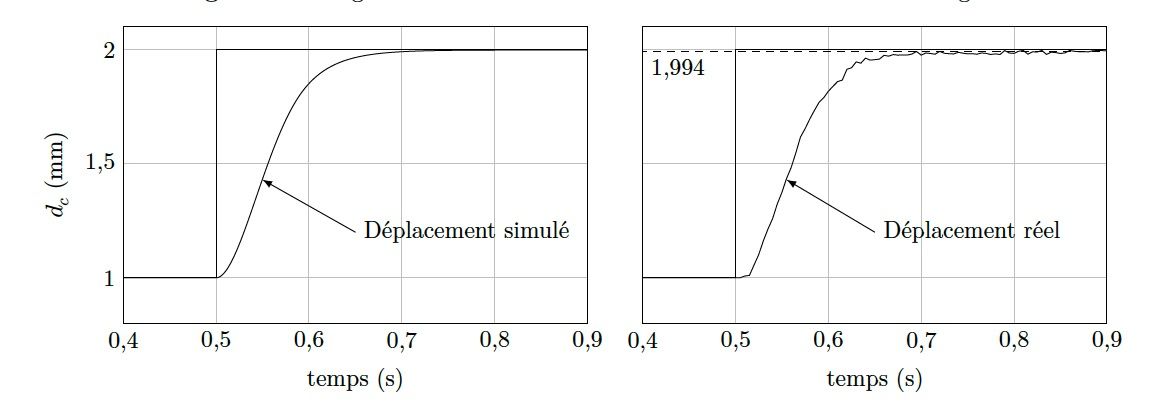
\includegraphics[width=1.0\textwidth]{images/image_simu.jpg}
\caption{Réponse indisielle finale simulée et réelle \label{fig_simu}}
\end{center}
\end{figure}




\subsection{Annexes}


Pour rappel : $u(t)$ est la fonction échelon unitaire.
\renewcommand\arraystretch{1.3}
\begin{center}
\begin{tabular}{|c|c||c|c|}
	\hline
	$f(t)$			&		$\displaystyle F(p)=\L\left[f(t)\right]$		&	$f(t)$				&	$F(p)=\L\left[f(t)\right]$			\\[0.3cm]
	\hline\hline
	$u(t)$			&		$\displaystyle \frac 1p$				&	$\sin(\omega t)\;u(t)$		&	$\displaystyle \frac{\omega}{p^2+\omega^2}$	\\[0.3cm]
	\hline
	$K\;u(t)$		&		$\displaystyle \frac{K}{p}$				&	$\cos(\omega t)\;u(t)$		&	$\displaystyle \frac{p}{p^2+\omega^2}$		\\[0.3cm]
	\hline
	$K\;t\;u(t)$		&		$\displaystyle \frac K{p^2}$				&	$\sinh(\omega t)\;u(t)$		&	$\displaystyle \frac \omega{p^2-\omega^2}$	\\[0.3cm]
	\hline
	$e^{-at}u(t)$		&		$\displaystyle \frac{1}{p+a}$				&	$\cosh(\omega t)\;u(t)$		&	$\displaystyle \frac{p}{p^2-\omega^2}$		\\[0.3cm]
	\hline
	$t^nu(t)$		&		$\displaystyle \frac{n!}{p^{n+1}}$			&	$e^{-at}\sin(\omega t)u(t)$	&	$\displaystyle \frac \omega{(p+a)^2+\omega^2}$	\\[0.3cm]
	\hline
	$e^{at} t^n u(t)$	&		$\displaystyle \frac{n!}{(p-a)^{n+1}}$			&	$e^{-at}\cos(\omega t) u(t)$	&	$\displaystyle \frac{p+a}{(p+a)^2+\omega^2}$	\\[0.3cm]
	\hline
	$\delta(t)$		&		$1$							&	$K\;\delta(t)$			&	$K$						\\[0.3cm]
	\hline
\end{tabular}
\end{center}
